\chapter{Agent Development Frameworks, SDKs, and Managed Runtimes}\label{ch:C22}
The October 2026 SDK releases expose failures that a framework comparison must represent. OpenAI Agents Python v0.24.0 defers automatic compaction while approvals are pending and preserves completed tool outputs when a sibling tool fails; Google ADK v2.13.0 marks its MongoDB session and memory services experimental~\cite{executionrelease02,executionrelease03}. These are version-specific documented changes, not guarantees inferred from a brand. They motivate comparing the exact interruption, publication, and compatibility semantics of a framework before counting its integrations.

An agent framework is a set of choices about where control resides. Its most consequential properties are not the number of model adapters or the expressiveness of a demonstration, but the semantics of state, effects, interruption, authorization, and observation. A framework can make those semantics explicit, hide them behind convenience interfaces, or delegate them to another service. These alternatives impose different experimental and operational obligations.

The comparison in this chapter begins with role rather than rank. A graph runtime, a typed model SDK, an opinionated harness, a workflow builder, and a managed execution platform occupy different boundaries. They can compose within one application and should not be treated as mutually exclusive competitors. The official-source inventory is interpreted as documentation of interfaces available for inspection on the literature cutoff, not as an independently stress-tested feature leaderboard.

\section{A semantic basis for framework comparison}\label{sec:C22:axes}
Define a framework profile by five sets: states it represents, transitions it controls, effects it mediates, observations it exports, and obligations it leaves to the application. This representation makes omissions visible. An SDK can validate a tool argument but leave external idempotency unspecified. A runtime can persist graph state but leave document authorization to a connector. A managed service can maintain sessions while exposing only partial execution traces. None of these limitations is inherently disqualifying; they determine the boundary of a defensible claim.

A useful comparison matrix distinguishes documented support from verified behavior. ``Persistence'' should be decomposed into conversation continuity, process-restart recovery, durable external artifacts, semantic memory, and cross-version migration. ``Human review'' should identify where execution pauses, what the reviewer sees, and whether authority is rechecked after resumption. ``Observability'' should identify whether traces include full tool arguments, truncation indicators, source identity, and asynchronous work. A single Boolean column loses these distinctions.

The unit of versioning is similarly broader than a package number. An application may combine a pinned SDK, moving model alias, remote tool schemas, hosted runtime, and changing connector permissions. Recording the SDK release alone does not reproduce the system. Define a compatibility vector whose components include each mutable boundary and attach it to evaluation traces. Unknown service revisions should remain unknown rather than be inferred from a documentation date.

More precisely, a configured deployment has a manifest $\xi=(\nu,\theta,\delta,\tau,\beta,\alpha)$: application/framework revision $\nu$, model identity $\theta$, deployment decoder $\delta$, tool-schema/adapter revision $\tau$, persistence backend/schema $\beta$, and current authority epoch $\alpha$. These components need not share a release cycle. A saved run additionally requires its realized context and external-effect records; $\xi$ identifies configuration rather than reconstructing those data. Framework comparison holds the relevant components fixed or declares their joint change as the treatment. Otherwise a newer SDK coupled to a stronger model is not an estimate of an SDK effect.

For feature equivalence, require observable contracts. Two frameworks both exposing a method called resume are not equivalent if one restores a model-visible history and another resumes an event-sourced workflow. The first may repeat tool effects; the second may skip completed activities but depend on deterministic application code. A conformance workload should therefore include an interruption after external acceptance and before local commitment, rather than test only that a suspended conversation can receive another message.

The practical implication is to select a framework against the failure modes of the intended workload. A short extraction service may benefit most from typed output and dependency injection. A multi-hour engineering task needs workspace state, cancellation, and reconciliation. A regulated business action needs principal identity and authoritative permission checks. Breadth of advertised features cannot replace the task-specific evidence needed to compare these roles.


\section{Graph runtimes and opinionated harnesses}\label{sec:C22:graphs}
Graph runtimes make control flow an explicit application object. Nodes transform state, edges constrain possible continuations, and persistence attaches to defined execution boundaries. This can support inspection and fault recovery, but the graph is not automatically deterministic: nodes can contain model calls, time-dependent queries, or external effects. A graph's visual clarity therefore does not prove replay equivalence. The implementation must identify which values are recorded and which computations execute again.

LangGraph illustrates a runtime layer, while Deep Agents supplies a more opinionated harness over that ecosystem~\cite{executionproduct001,executionproduct006}. The latter's documented filesystem, subagent, and context-management interfaces are mechanisms to examine. Their existence does not establish that summaries preserve every constraint or that delegated work is cheaper. A useful experiment holds the underlying runtime fixed and separately varies offloading, compaction, and delegation. Otherwise a comparison between the two layers confounds control defaults with the runtime itself.

An opinionated harness reduces application effort by choosing defaults for prompts, tools, memory, and stopping. The benefit is faster construction of a coherent system. The scientific cost is that a high-level configuration can activate several mechanisms at once. Researchers should expose these defaults in their experimental configuration and inspect the code path used by the evaluated task. Disabling a component should not silently activate a fallback whose cost or behavior is materially different.

Event-driven workflow systems provide another control model. Events describe completed work or new requirements, and handlers may schedule further tasks. This is useful when external processes, human decisions, or delayed data determine progress. However, event duplication and ordering become part of agent semantics. A workflow that processes the same approval event twice can execute an action twice unless it deduplicates by stable event identity. These concerns persist even if every model call is perfectly accurate.

The discriminating experiment is not whether a sample application runs. It is whether equivalent state transitions produce equivalent committed effects under interruptions, retries, and schema evolution. Use a small deterministic tool fixture first, then introduce model nondeterminism as a separate factor. This ordering prevents a transport or persistence defect from being misdiagnosed as reasoning failure. It also establishes which guarantees survive when the framework delegates execution to a managed backend.


\section{Typed SDKs and model-owned loops}\label{sec:C22:typed}
Typed SDKs place schemas and application dependencies around model interactions. Type validation can reject malformed arguments, constrain output shape, and expose errors before application code executes. Its guarantee is syntactic and representational. A valid customer identifier can still refer to the wrong customer, and a well-typed monetary amount can still exceed authorization. Semantic preconditions must therefore remain explicit application checks rather than be assumed consequences of schema adherence.

The inspected OpenAI Agents SDK separates an application-owned SDK path from managed runtime options~\cite{openai2026agents}. Handoffs, tool loops, session interfaces, and tracing provide useful abstractions, but applications still own tool effects and their storage semantics. Its SDK is provider-agnostic; the evaluation must identify the selected model adapter rather than infer it from the SDK name~\cite{executionproduct002}. PydanticAI makes typed interaction an inspectable design surface and also supplies a configurable harness, while Pydantic Graph and Pydantic Evals are separate packages~\cite{executionproduct004}. Restricting its inventory to output validation would omit its current context, tool and execution controls. A comparison should examine how validation failures are surfaced, whether repair attempts consume the same budget, and whether rejected calls enter the trajectory used for later training or evaluation.

The Claude Agent SDK occupies a different ownership boundary from a Messages API client. Current official documentation describes a Python/TypeScript library running the Claude Code binary in an application-operated process, with its agent loop, tool execution, permissions, sessions and hooks. A client SDK instead exposes model requests, while Claude Managed Agents supplies a hosted harness with a separately configured execution environment~\cite{cumb2026claudesdk,executionproduct061}. These are three distinct experimental treatments. A common model identifier does not make their context constructors or permission mechanisms equivalent.

One failure mode is repair-induced drift. A model proposes an invalid tool call, the SDK returns an error, and the next attempt changes a meaningful argument while correcting the format. If evaluation records only the final valid call, it omits the information that caused the transition. For a learned policy this can invalidate behavior-likelihood reconstruction. For a production service it can conceal repeated boundary probing. Validation and repair events should therefore be first-class trace records.

Model-owned loops choose their next action dynamically, whereas application-owned workflows constrain the available continuation structure. Neither is universally superior. Dynamic loops accommodate unforeseen subtasks but can cycle, invent unsupported tool names, or consume budgets without progress. Explicit workflows improve predictability but can fail when the task falls outside their branches. A hybrid design uses deterministic control for authority and commitment while permitting model-driven choice within a bounded action space.

The relevant baselines compare the same tool contract under direct function orchestration, a minimal agent loop, and the SDK's higher-level abstractions. Measure invalid calls, repair rounds, constraint violations, total cost, and completion. A framework's ergonomic advantage is real but requires a different study, such as developer implementation time under controlled tasks. It should not be inferred from task success or substituted for runtime reliability.


\section{Development kits interoperability and language boundaries}\label{sec:C22:adks}
An agent development kit typically bundles authoring conventions, tool integration, orchestration, testing, and deployment adapters. This breadth can improve consistency but also creates version coupling. A task object serialized by one language implementation may not preserve every field expected by another. A model adapter can normalize errors differently, changing retry behavior. Cross-language support is therefore a compatibility question rather than a guarantee that all implementations have identical semantics.

Google ADK's inspected repository describes graph-based workflows and structured delegation surfaces, while Microsoft Agent Framework describes multi-language agent and workflow construction~\cite{executionproduct003,executionproduct007}. These are concrete interfaces for conformance tests. The experiment should pin the relevant implementation and compare equivalent task graphs, state updates, and failure injections. It should not compare unrelated examples and attribute the difference to the toolkit brand.

Protocol support is similarly conditional. A framework advertising MCP can expose tools, resources, or prompts through different transport and authorization configurations. An A2A integration can exchange task status without sharing the same memory model or trust boundary. Chapter~\ref{ch:C19} treats these protocol distinctions directly. At the framework layer, the important question is which semantics are preserved when an adapter maps between local objects and external messages.

Serialization requires particular care for authority-bearing data. A human approval record should identify the precise operation, relevant arguments, principal, expiry, and policy epoch. Mapping it to an unstructured string in another framework weakens its meaning. The receiving application must validate the approval against its own action boundary. Successful message delivery cannot establish that the transferred object authorizes the requested effect.

Interoperability experiments should include a deliberate version mismatch, optional fields unknown to the receiver, partial tool failures, and revoked credentials. Report which failures are detected before dispatch and which emerge only after an effect. A graceful error is often preferable to a silent fallback that changes task meaning. The strongest interoperability result is a documented set of preserved invariants under declared adapters, not an assertion that any agent can collaborate safely with any other.


\section{Role-specific framework and runtime inventory}\label{sec:C22:inventory}
Table~\ref{tab:C22:inventory} assigns each listed framework or managed runtime a concrete inspection target. The entries describe documentation surfaces, not measured capability or comparative quality. The final column is a discriminating test: it identifies an observation needed before an engineering conclusion is justified. Where a source redirects, the resolved resource defines the inspected family; historical names are lineage identifiers. Package and hosted-service parity remain unverified unless established by a version-specific test.
\begingroup\setlength{\tabcolsep}{3pt}\small
\bookneedspace{.42\textheight}
\begin{longtable}{L{25mm}L{35mm}L{48mm}}
\caption{Framework and managed-runtime surfaces with discriminating checks.}\label{tab:C22:inventory}\\
\toprule Product & Documented surface & Required test \\
\midrule\endfirsthead
\toprule Product & Documented surface & Required test \\
\midrule\endhead
LangGraph\cite{executionproduct001} & Graph checkpoints and stores & Crash after an effect; distinguish restored state from repeated dispatch. \\
OpenAI Agents SDK\cite{executionproduct002} & Agent and Runner loop interfaces & Preserve rejected calls, handoff ownership and application side-effect receipts. \\
Agent Development Kit — ADK\cite{executionproduct003} & Workflow and task delegation objects & Compare graph transitions under retry, human interruption and version mismatch. \\
PydanticAI\cite{executionproduct004} & Typed loop and configurable harness & Inject validly typed but unauthorized arguments; separate types from permission checks. \\
Deep Agents\cite{executionproduct006} & Filesystem offload and isolated subagents & Remove a rare constraint during compaction and test later recovery. \\
Microsoft Agent Framework\cite{executionproduct007} & Multi-language agents and workflows & Round-trip state across language adapters; retain cancellation and error semantics. \\
Agno / AgentOS\cite{executionproduct010} & Agent teams and runtime interfaces & Test whether shared memory commits conflict or silently overwrite one another. \\
LlamaAgents / Agent Workflows\cite{executionproduct011} & Event-driven workflow composition & Duplicate an input event and inspect whether downstream effects repeat. \\
Strands Agents / Harness SDK\cite{executionproduct012} & Composable harness control interfaces & Locate the actual agent-loop implementation after the source redirect; pin the adapter. \\
OpenClaw\cite{executionproduct014} & Cross-channel agent gateway & Revoke one channel principal and test isolation of historical context. \\
Mastra\cite{executionproduct019} & TypeScript agents and workflows & Interrupt a suspended workflow and verify that resumption preserves evidence identity. \\
Claude Agent SDK\cite{executionproduct020} & Claude-oriented SDK execution surfaces & Identify application versus provider ownership of hooks, session state and tool effects. \\
Haystack\cite{executionproduct026} & Retrieval pipelines and agent components & Replace retrieval with oracle evidence while holding generation and tool budgets fixed. \\
NeMo Fabric\cite{executionproduct031} & Cross-harness execution and telemetry & Check whether adapter traces preserve truncation, delegated work and error provenance. \\
smolagents\cite{executionproduct032} & Code-action agent loop & Inspect the generated-code execution boundary and sandbox mediation of effects. \\
DeepSeek Harness\cite{executionproduct035} & Plugin-oriented harness interfaces & Disable one plugin and inspect transitive tool exposure and persisted assumptions. \\
AgentScope\cite{executionproduct039} & Agent application and team abstractions & Test cancellation propagation and whether conversation identifiers imply durable storage. \\
CrewAI\cite{executionproduct041} & Role-based crews and explicit flows & Compare identical role assignments with deterministic flow and model-selected delegation. \\
Pi\cite{executionproduct049} & Terminal harness and extension interfaces & Load a minimal extension and audit which credentials and context it receives. \\
DSPy\cite{executionproduct052} & Program optimization against evaluation & Keep an untouched holdout and count selection attempts as part of optimization cost. \\
OGX, formerly Llama Stack\cite{executionproduct054} & Portable server-side agent interfaces & Follow the OGX lineage and verify old client schema compatibility explicitly. \\
Qwen-Agent\cite{executionproduct056} & Qwen-oriented tools and retrieval & Match tool serialization and model settings before attributing benchmark differences. \\
n8n\cite{executionproduct057} & Workflow automation with agent steps & Separate durable workflow state from model-visible memory and connector permissions. \\
Langflow\cite{executionproduct062} & Visual Python agent composition & Export the executable graph and test whether visual and API paths agree. \\
Dify\cite{executionproduct066} & Visual workflows and retrieval pipelines & Check which runtime and connector components are actually inspectable and licensed. \\
Elastic Agent Builder\cite{executionproduct068} & Search-grounded agent construction & Change document permissions after indexing and test retrieval-time enforcement. \\
CAMEL\cite{executionproduct071} & Collaborating agent framework & Compare communicating workers against equal-cost independent samples and one-agent controls. \\
Coze Studio\cite{executionproduct082} & Self-hostable visual agent workflows & Inspect credential scoping, deployment dependencies and duplicate-event recovery. \\
UiPath Maestro\cite{executionproduct018} & Business-process orchestration patterns & Interrupt a human approval chain; bind the resumed action to current authorization. \\
Agent Bricks\cite{executionproduct042} & Custom-agent hosting and data integration & Verify workspace persistence and trace identity across a container restart. \\
Bedrock AgentCore\cite{executionproduct043} & Composable runtime identity and memory services & Test service boundaries separately; a memory feature does not establish agent correctness. \\
Gemini Enterprise Agent Platform\cite{executionproduct044} & Managed agent lifecycle services & Distinguish low-code, managed API and custom ADK deployment semantics. \\
Agents API\cite{executionproduct060} & Managed sessions and execution harness & Compare saved turn history with actual external-effect reconciliation under failure. \\
Claude Managed Agents\cite{executionproduct061} & Managed long-running agent sessions & Inspect environment persistence, permission policy and incomplete-turn outcomes independently. \\
Agents \& Conversations API\cite{executionproduct089} & Agent configuration and conversation entries & Test history continuity separately from tool execution and external transaction guarantees. \\
\bottomrule\end{longtable}
\endgroup


Several entries cross category boundaries. Pi can be used as a coding harness and as an extension substrate. NeMo Fabric concerns execution and telemetry across harnesses rather than a replacement for the model policy. DSPy concerns program and prompt optimization against evaluation objectives; it should be tested for selection overfitting as well as task quality. A visual builder such as Langflow, Dify, Coze Studio, or n8n can host model-driven steps inside deterministic workflows. Its graphical interface does not remove the need to examine stored state, credential scope, and replay behavior.

Managed platforms change the observation boundary. AgentCore, Agent Bricks, and Google's enterprise platform document infrastructure surfaces that an application can compose with custom agents. Managed agent APIs supply a larger portion of the loop. These roles should be compared through migration effort, observability, failure recovery, and enforceable policy controls, rather than counted as additional reasoning architectures. A serverless runtime's availability commitment is not evidence that an agent's task output is correct.


\section{Licensing lifecycle and migration evidence}\label{sec:C22:lifecycle}
Implementation visibility, artifact license, hosted-service terms, and operational inspectability are separate properties. A public repository can contain a client while the service remains proprietary. A source-visible license can restrict deployment or redistribution. A permissive core license may coexist with separately licensed connectors or enterprise features. The defensible statement identifies the inspected artifact and its license file at a revision; it does not attach an unqualified open-source label to an entire product family.

The inspected repository notices illustrate why this granularity matters. Mastra distinguishes its Apache-2.0 core from enterprise-licensed directories; n8n identifies Sustainable Use and Enterprise licenses; Dify identifies an Apache-2.0-derived license with additional conditions~\cite{executionproduct019,executionproduct057,executionproduct066}. These notices establish artifact-specific terms, not a universal compatibility judgment between deployments. DeepSeek Harness explicitly declares developer-preview status and anticipated compatibility-breaking changes~\cite{executionproduct035}. An active commit stream therefore does not establish a stable serialized-state or plugin ABI.

Lifecycle changes can invalidate comparisons even when names remain familiar. The inspected Llama Stack link resolves into the OGX lineage, and the Llama workflow link resolves to a broader agents repository. The Strands source link resolves to a harness SDK resource. These redirects are evidence of naming and packaging changes, not proof of complete backward compatibility. An application relying on old imports, storage schemas, or tool names needs a migration test rather than a renamed bibliography entry.

Historical products should be preserved where they explain architectural evolution, but they should not be described as active recommendations without current evidence. Archive status, maintenance activity, security-fix policy, and availability are distinct. A repository can remain readable after service termination; a commercial service can remain available while a legacy SDK is deprecated. The operating consequence is to maintain a dependency inventory with replacement and rollback plans, particularly for long-lived memory formats.

A migration experiment starts from a saved run and its authoritative state. Restore under the target release, validate schemas, rebuild indexes when required, and replay deterministic fixtures before permitting new model decisions. Compare tool availability, parser behavior, serialization, and cancellation. A test that merely imports the new package misses the semantics most likely to affect agent behavior. If the provider does not expose the necessary version controls, report that reproducibility limitation explicitly.

For a deterministic fixture, write $F_\nu:\mathcal S_\nu\times\mathcal U\to\mathcal S_\nu$ for a release's state transition and $O_\nu:\mathcal S_\nu\times\mathcal U\to\mathcal E$ for its observable event output. Let $m:\mathcal D\subseteq\mathcal S_\nu\to\mathcal S_{\nu'}$ be a partial migration with the same fixture inputs $\mathcal U$. On a transition-closed migration domain, require
\begin{align}
 m(F_\nu(s,u))&=F_{\nu'}(m(s),u),\\
 O_\nu(s,u)&=O_{\nu'}(m(s),u).
 \label{eq:C22:migration_commutes}
\end{align}
If both identities hold for every admitted $(s,u)$, induction on the finite input sequence gives identical fixture event traces and corresponding states after every step. This is a contract-preservation criterion, not a claim that all migrations satisfy it. The event space must include relevant tool intents, validation failures and recorded receipts; comparing only final chat strings discards precisely the events that can change effects. Real remote effects still require the service contract of Chapter~\ref{ch:C20}. A migration may legitimately reject an unsupported saved state; silently coercing it into another agent's state violates the criterion. A finite test suite provides evidence on its reached states, not proof of the universal identities. Stochastic model transitions require distributional comparison or fixed recorded outputs, rather than assuming identical samples.

Ownership and acquisition claims are excluded from technical inference unless primary evidence establishes them and they matter to the system boundary. Even a verified corporate change does not imply that products share code, data, or runtime guarantees. The analysis follows inspectable mechanisms and contracts. This avoids turning a provider map into an unsupported architectural map.


\subsection{Release-specific evidence at the October cutoff}
The official release records rechecked on 29 October identify LangGraph 1.2.18 on 26 October 2026, OpenAI Agents Python SDK 0.24.0 on 15 October, Google ADK 2.13.0 published on 23 October with release-note heading dated 22 October, and PydanticAI 2.63.0 on 28 October\cite{executionrelease01,executionrelease02,executionrelease03,executionrelease04}. These identifiers delimit the evidence; a current main branch can contain later or unreleased changes. Microsoft's repository has distinct .NET 1.26.0 and Python 1.23.0 releases, dated 23 and 22 October respectively, rather than one universal cross-language release\cite{executionrelease05,cumb2026mafpython}. CrewAI's inspected release was 1.15.32, while smolagents' latest returned release was 1.26.0 from May\cite{executionrelease07,executionrelease06}. Release recency alone is not a quality metric.

Several changes directly affect the consistency arguments in this book. LangGraph's notes change the default frequency of full delta snapshots from one thousand updates to one hundred, trading additional storage for faster reads on long threads. This is a concrete checkpoint-layout change, not evidence of better semantic memory. The Agents SDK notes defer automatic compaction during pending approvals, replace Redis compaction history atomically, and preserve completed tool outputs when a sibling fails. Those fixes identify distinct state boundaries: approval evidence, history replacement and partial parallel completion. They motivate targeted regression fixtures rather than a general claim that all consistency problems are solved\cite{executionrelease01,executionrelease02}.

ADK's release notes mark MongoDB session and memory services experimental even while promoting other features to stable status. They also change the default telemetry schema. Consequently, neither maturity nor trace compatibility should be assigned at whole-framework granularity. An analytics pipeline that assumes an older span layout can silently lose attribution after an otherwise successful upgrade. PydanticAI's notes change the default of its \texttt{CodeMode} dynamic catalog so newly revealed tools append rather than rewrite cached prompts. That is a component-specific context-construction choice whose effect depends on tool-discovery workload and cache behavior; it is not a universal change to every tool path or a measured application-level speedup\cite{executionrelease03,executionrelease04}.


Figure~\ref{fig:C22:overview} isolates the mechanism and its stated information boundaries.
\begin{figure}[!htbp]
\centering
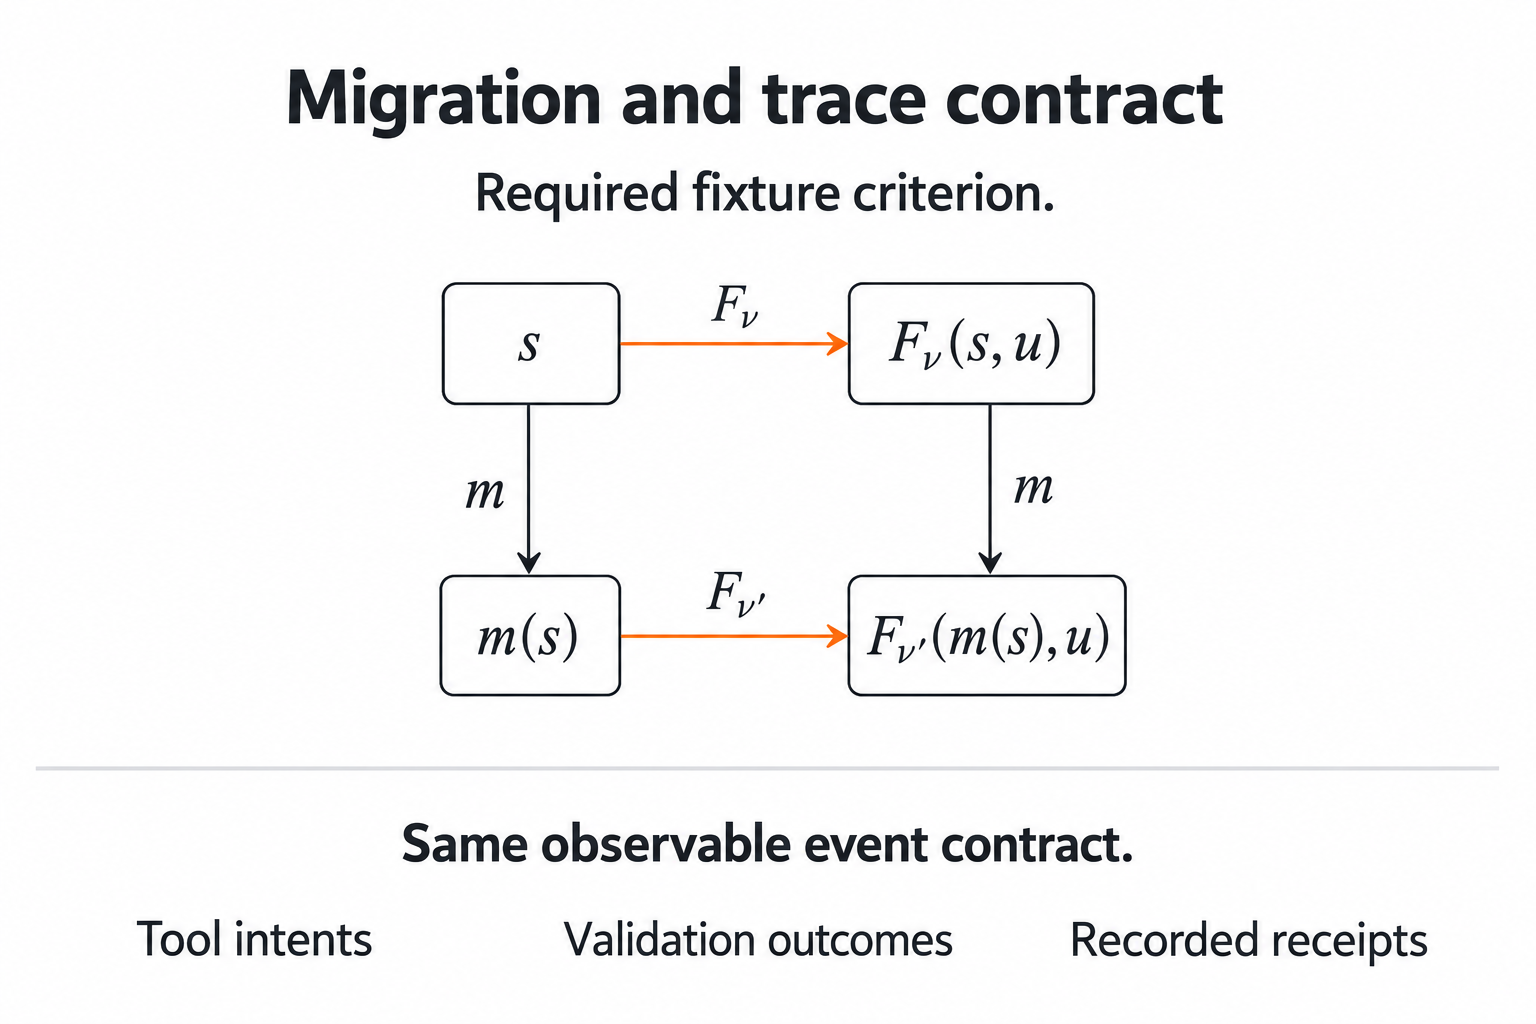
\includegraphics[width=\linewidth]{book/figures/assets/F22review.png}
\caption{A deterministic migration criterion compares the two paths through corresponding fixture states. On an admitted transition-closed domain, migration must commute with the state transition and preserve the declared observable events. Finite fixtures test reached states; they do not prove the universal identities or establish remote-effect uniqueness.}
\label{fig:C22:overview}
\end{figure}

\section{A conformance suite before performance ranking}\label{sec:C22:conformance}
A framework conformance suite should exercise schema validation, state restoration, duplicate dispatch, cancellation, authorization revocation, and trace completeness before comparing task scores. Each fixture has an expected observable contract. For example, a revoked write capability must prevent a new effect even if an old checkpoint contains a permission statement. A committed terminal receipt should be replayed without a new effect; an unresolved dispatch should reconcile before any retry justified by the service's explicit retry contract. A truncated tool result should carry an explicit truncation indication or preserve a recoverable artifact reference.

Conformance is not a universal safety certificate. It establishes behavior for the tested contract and release. A framework can pass deterministic fixtures and still induce poor model decisions through context construction. Therefore the second stage evaluates task outcomes under matched models, tools, and budgets. Separate the effect of the framework from the effect of its recommended prompt, default model, and hosted extensions. When those cannot be separated, the treatment is the complete configured system.

Component effects need not be additive. For two configurable mechanisms, let $\mu_{ij}$ be expected task outcome when mechanism one has state $i\in\{0,1\}$ and mechanism two has state $j\in\{0,1\}$, with the backbone, information access, resource envelope and task population fixed. The interaction is
\begin{equation}
 I=\mu_{11}-\mu_{10}-\mu_{01}+\mu_{00}.
\end{equation}
For example, compaction can change which tool descriptions remain visible, while dynamic discovery changes which descriptions need to survive compaction. A gain from enabling both does not identify either individual contribution; a nonzero $I$ measures their departure from additivity on the declared outcome scale. If an SDK cannot expose all four configurations, the interaction is unidentified from that product comparison. This is an explicit observation limit, not a reason to assign the combined gain to the most prominently advertised feature.

Statistical comparisons should use paired tasks and report uncertainty at the task or session level. Framework adapters can fail only on particular tool schemas, so stratify by schema complexity and effect type. Count startup failures, missing outputs, and dependency outages rather than removing them as setup problems after observing results. A system that requires undocumented manual repair has a materially different operational profile from one that completes unattended under the same fixtures.

Finally, include an implementation-complexity analysis without mistaking it for benchmark quality. Count application-owned components, external dependencies, state stores, custom adapters, and recovery code. These counts do not form a universal simplicity score, but they explain where maintenance responsibility resides. A highly capable managed service may reduce local code while increasing opaque dependencies. A minimal SDK may expose more work but permit a stronger audit. The appropriate choice depends on which uncertainty the deployment can tolerate and which guarantees it must enforce.

\section{From public API to executable control path}\label{sec:C22:codepaths}
A concrete audit can start with three interfaces rather than an entire framework taxonomy. In the inspected LangGraph source tree, the state-graph implementation resides in the graph state module and exposes compilation into an executable graph. In the OpenAI Agents Python SDK, the run module exposes the Runner control surface. The Google ADK source exposes runner infrastructure for application execution. These are identifiable inspection points, not assertions that the corresponding modules implement every guarantee discussed above. Their current source files were reachable at the cutoff; experiment revisions still require immutable pinning~\cite{executionproduct001,executionproduct002,executionproduct003}.

For the graph case, trace compilation into checkpoint use. Identify where thread identity enters configuration, which state updates are reduced together, and which node outputs are persisted before successors execute. Then place an effectful tool call inside one node and inject a crash immediately after the service accepts it. If resumption reexecutes the node, the application must supply idempotency or reconciliation. This test distinguishes graph-state durability from external-effect uniqueness without requiring a language model in the fixture.

For the Runner case, trace model output through tool-call decoding, schema validation, execution, and subsequent model input. Capture the exact error object returned for an invalid argument. Then inspect whether a handoff changes the active instructions, tools, model settings, or state ownership. The experiment should preserve the pre-handoff authority envelope and verify that delegation cannot expand it. A handoff that routes a conversation successfully can still be incorrect if it transfers more context or credentials than the receiving specialist requires.

Current source inspection supplies narrower testable claims. LangGraph's pinned \path{DeltaChannel} constructor sets \texttt{snapshot\_frequency=100}; this supports the checkpoint-layout claim without asserting semantic preservation by compaction~\cite{cumb2026langgraphcode}. The Agents SDK's pinned \path{RunState} uses schema 1.21 and rejects ambiguous legacy agent identities; its documentation warns that neither context overrides nor strict context deserialization establishes snapshot integrity~\cite{cumb2026agentsstate}. The required fixture therefore changes a duplicate-agent graph and verifies a safe rejection, rather than relabeling an old checkpoint until loading succeeds. Serialization compatibility and authenticity are separate checks.

For an ADK application, inspect how an event updates session state and how workflow execution consumes that state. Duplicate one event identifier and delay another. The expected behavior must come from the selected application's contract, because a generic toolkit may legitimately expose several scheduling modes. Evaluate whether the serialized event contains sufficient identity to diagnose the difference. A toolkit's flexibility increases the number of legal configurations; it does not eliminate the need to state which one produced a result.

For example, the pinned ADK \path{InMemorySessionService.append_event} skips partial events and suppresses an equal re-delivery only after matching its event identifier. Distinct event objects with the same identifier but different fields are retained. Its scope is an in-memory session implementation, not restart durability or universal event-ID uniqueness across backends~\cite{cumb2026adksession}. A discriminating fixture must therefore test both identical re-delivery and conflicting reuse, and must inspect the selected persistent backend independently. An identifier's presence in a serialized object is insufficient evidence that every consumer enforces its intended uniqueness.

These inspections produce a claim-to-code ledger. Each row records the public claim, source revision, module and callable, relevant configuration, injected condition, expected invariant, and observed outcome. Until the fixture has run, the outcome field remains unmeasured. This restraint prevents source inspection from becoming an invented reproduction. When the experiment does run, a discrepancy should lead to a narrower conclusion: perhaps a configured checkpointer preserves local state, while the selected tool adapter repeats effects. Blaming or endorsing the entire framework would discard the evidence about where the behavior actually arose.

The ledger also identifies work needed for upgrades. If a release changes the callable responsible for event reduction or tool retries, rerun the fixtures attached to those claims. An unrelated documentation edit need not trigger all experiments. This dependency-based approach makes validation scalable while retaining scientific traceability. It is especially useful for agent systems because a small change to error serialization can alter the model's next action even when the application's visible API remains compatible.

